\documentclass[a4paper,11pt]{article}

\usepackage[T1]{fontenc}
\usepackage[utf8]{inputenc}
\usepackage{graphicx}
\usepackage{xcolor}
\usepackage[fleqn]{amsmath}
\usepackage{tgtermes}
\usepackage[final]{pdfpages}

\usepackage[
pdftitle={Lingwistyka Formalna i Automaty},
pdfauthor={evemorgen, AGH},
colorlinks=true,linkcolor=blue,urlcolor=blue,citecolor=blue,bookmarks=true,
bookmarksopenlevel=2]{hyperref}
\usepackage{amsmath,amssymb,amsthm,textcomp}
\usepackage{enumerate}
\usepackage{multicol}
\usepackage{tikz}
\usepackage{geometry}
\geometry{
 a4paper,
 total={170mm,257mm},
 left=20mm,
 top=20mm,
}

% custom footers and headers
\usepackage{fancyhdr,lastpage}
\pagestyle{fancy}
\lhead{}
\chead{}
\rhead{}
\lfoot{Assignment \textnumero{} 2}
\cfoot{}
\rfoot{Page \thepage\ /\ \pageref*{LastPage}}
\renewcommand{\headrulewidth}{0pt}
\renewcommand{\footrulewidth}{0pt}
%

%%%----------%%%----------%%%----------%%%----------%%%

\begin{document}

\title{Lingwistyka Formalna i Automaty - ćwiczenia 2}
\author{evemorgen, AGH}
\date{20/11/2016}
\maketitle

\newpage
\section{Podać DAS, które akceptują poniższe języki nad alfabetem \{0,1\}:}
\subsection{Zbiór wszystkich łańcuchów zawierających podłańcuch '101'}
\begin{center}
	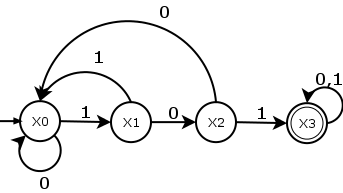
\includegraphics[]{1a}
\end{center}

\subsection{Zbiór wszystkich łańcuchów zaczynających się od '1' i kończących się na '1'}
\begin{center}
	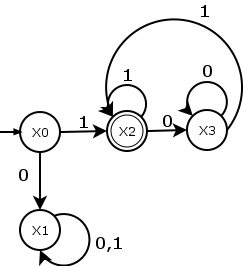
\includegraphics[]{1b}
\end{center}

\subsection{Zbiór wszystkich łańcuchów zaczynających się od '0' i kończących się na '0'}
\begin{center}
	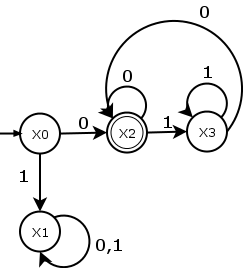
\includegraphics[]{1c}
\end{center}

\subsection{Zbiór wszystkich łańcuchów zaczynających się od '0' lub '1' i kończących się na '1'}
\begin{center}
	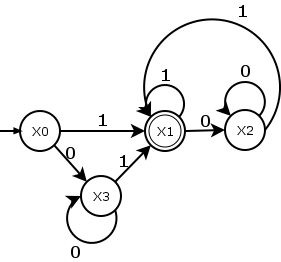
\includegraphics[]{1d}
\end{center}

\subsection{Zbiór wszystkich łańcuchów zawierających podłańcuch '001'}
\begin{center}
	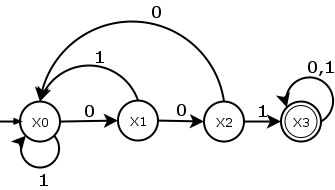
\includegraphics[]{1e}
\end{center}

\subsection{Zbiór wszystkich łańcuchów kończących się '00'}
\begin{center}
	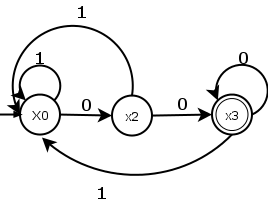
\includegraphics[]{1f}
\end{center}

\subsection{Zbiór wszystkich łańcuchów zawierających '000'}
\begin{center}
	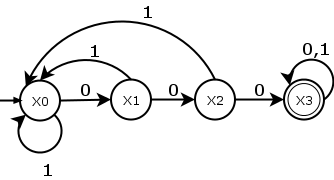
\includegraphics[]{1g}
\end{center}

\subsection{Zbiór wszystkich łańcuchów mających '1' na trzeciej pozycji od końca}
\begin{center}
	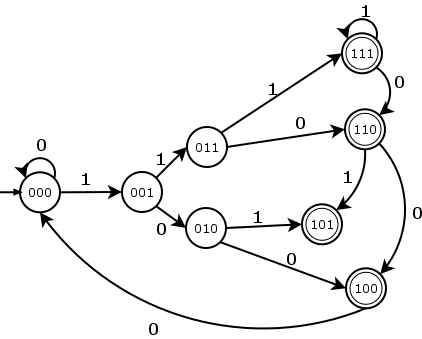
\includegraphics[]{1h}
\end{center}

\newpage
\section{Opisać jaki język akceptują poszczególne DAS:}
\subsection{}
\begin{center}
  \includegraphics[]{tab1}
  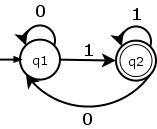
\includegraphics[]{2a} \\
  \huge
  Zbiór wszystkich łancuchów kończących się na 1
\end{center}
\subsection{}
\begin{center}
  \includegraphics[]{tab2}
  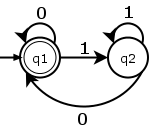
\includegraphics[]{2b}
\end{center}
  \huge
  Zbiór wszystkich łancuchów kończących się na 0 i  pusty string.

\newpage
\subsection{}
\begin{center}
  \includegraphics[]{tab3}
  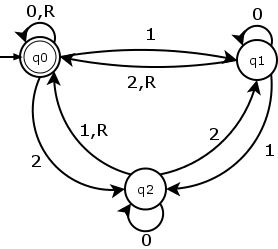
\includegraphics[]{2c}
\end{center}
  \huge
  Zbiór wszystkich łańcuchów złożonych z cyfr których suma modulo 3 jest równa 0.

\newpage
\section{Opisać jaki język jest akceptowany przez $\varepsilon$-NAS:}
  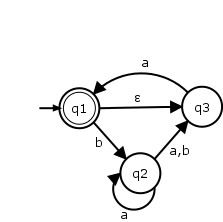
\includegraphics[]{enas1}
  \huge
   Wszystkie łańcuchy składające się ze znaków '0'  których jest $2n$ lub $3n$ gdzie $n \in \mathbb{N}$ (akceptowalny jest również pusty łańcuch)

\newpage
\section{Dany jest $\varepsilon$-NAS}
\includegraphics[]{tab4} \\

Rozrysować jego działanie dla łańcuchów:
\begin{itemize}
	\item 010110
    \item 101001
    \item 000111
    \item 111000
\end{itemize}
\subsection{010110}
\begin{center}
	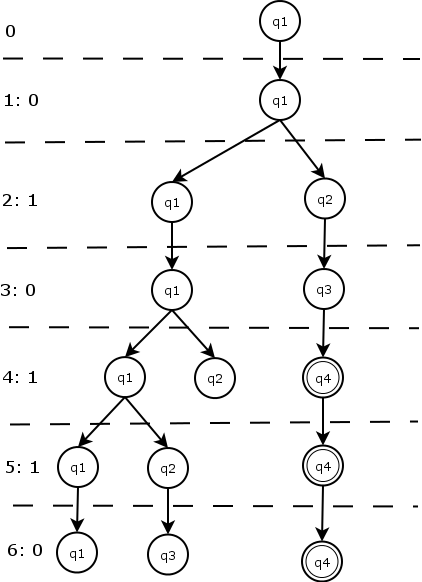
\includegraphics[]{4a}
\end{center}

\subsection{101001}
\begin{center}
	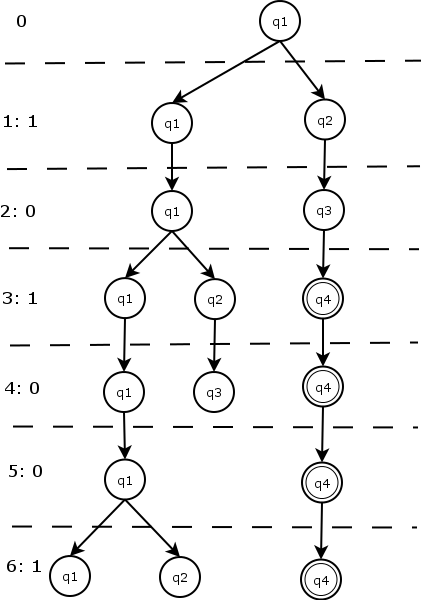
\includegraphics[]{4b}
\end{center}

\subsection{000111}
\begin{center}
	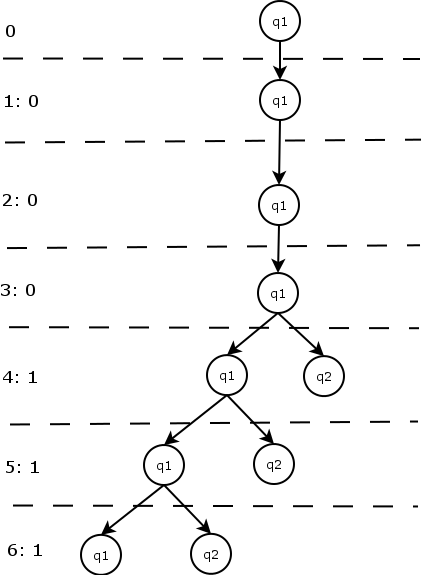
\includegraphics[]{4c}
\end{center}

\subsection{111000}
\begin{center}
	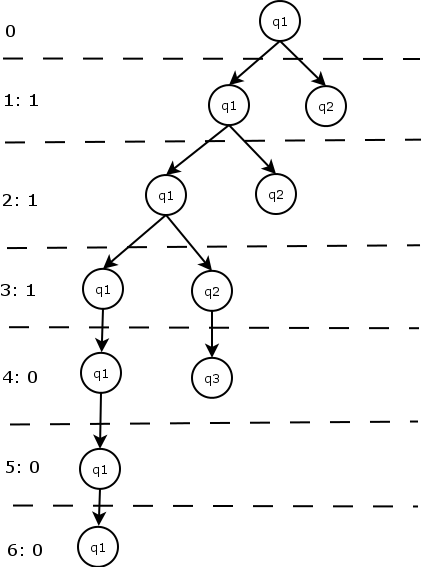
\includegraphics[]{4d}
\end{center}

\end{document}
